\chapter{Introduction}
%$$\mu$ 
\section{There is an increasing scientific and biomedical need for low-input nucleic acid analyses}

Applications from microbial genome discovery to biomedicine\cite{Blainey:2013hn,Marshall:2012jz,Wang:2012bb,Huggett:2015hp,Evrony:2016du,Evrony:2012dl,Rinke:2013bt,Navin:2011jq} are driving the broader application of high-throughput analyses of nucleic acids at the level of single molecules and single cells. In this introduction, I will describe the specific scientific and biomedical needs for single-molecule and single-cell analyses in the characterization of unculturable microorganisms, human microbiome research, cancer research, and clinical diagnosis. Following that, I will discuss the related technology landscape and ideal functionalities for such analyses. Lastly, I will preview my technology, \textit{virtual microfluidics}, which is the focus of this thesis. I will explain how this technology fits in the emerging single-cell field and discuss its potential to provide significant improvement and value in enabling easily accessible, high-quality, and low-input genomic research to a large scientific and biomedical field. 

\subsection{Characterizing unculturable microorganisms needs single-cell sequencing}

Microbial communities (including bacteria and archaea) and their globally distributed networks are an essential part of human life on earth. They are highly diverse, with an estimated $10^{7}$ prokaryotic species \cite{Curtis:2002dj}. These microbes play critical roles in ecosystems that break down sewage, produce beer at an industrial scale, and associated with` human health. For example, \textit{D. radiodurans} was first discovered in soil as the most radiation-resistant organism known. It was then engineered with toluene dioxygenase to survive in highly radioactive waste sites and decompose hazardous chemicals such as toluene and chlorobenzene \cite{Lange:1998ea}. Also, it has been shown that long-term antibiotic treatment causes prolonged shifts in the gut microbial composition, which decreases amyloid$\beta$ plaque deposition and is associated with the Alzheimer's disease in human \cite{Minter:2016ga}. Despite their importance, 90-99\% of microbes have not been characterized because they are difficult to culture in the lab \cite{Yilmaz:2011bc}. Studying the uncharacterized microorganisms can open the door to the huge reservoir of knowledge on microbial functions and gives us the ability to predict microbial responses to perturbations from human activities.  

%A better understanding of the microbial communities could help improve industry-scale production, bioremediation of industry effluent and oil spill \cite{Maulin:2017wy,Roling:2002vi} and give us the ability to predict response to perturbations \cite{Hamamura:2006iz,Minter:2016ga}. 
% from angela I think you should go one step further and provide 1-2 concrete examples of how a better understanding of microbial behavior will impact the applications you mention. Maybe write 'For example,...' and then include a specific example of how this will impact bioremediation or therapeutics. 
% It is also critical to predict microbial responses to perturbations from human activities.

The highly diverse nature of environmental microbes, however, requires the characterization of the microbe in isolation. Studying microbes in this way is needed in order to understand the individual microbe's physiology and relationship with different components of its community. Traditional methods of isolating a single species in culture are not only labor-intensive and slow, but they also require serial enrichment under culture conditions that are often sub-optimal for microbes' growth\cite{Blainey:2013dp}. Such a prolonged procedure increases the risks of genomic changes in the microbe of interest and may result in diversity loss due to competition or simple unculturability. Meanwhile, optimizing the culture conditions for a large number of diverse species of bacteria is difficult. 
Understanding the metabolic mechanism of an uncharacterized microbe could shed light on an axenic culture in the lab and in many cases, a symbiotic co-culture might be necessary \cite{HuiWang:2014gj}. 
% think you could add 1-2 more sentences that are more detailed about the challenges of uncultured organisms in this section.

To address these issues, the recent development of next-generation sequencing techniques has enabled us to discover a large number of microorganisms \cite{Rinke:2014fu,Stepanauskas:2007ir}. Specifically, these sequencing techniques have allowed scientists to identify the functional pathways and phylogenies of newly characterized microorganisms \cite{Rinke:2013bt}. Furthermore, the evolutionary history and relationships among prokaryotic species are developed based on marker genes, such as 16S sequences, instead of solely relying on qualitative morphology observations. 

Recent studies have discovered new variations of genetic code encoding for amino acids. Across the diversity of microbes, the genetic code for amino acids has been shown to vary in size and codon assignment\cite{Prat:2012ef}. UGA is a common stop codon. A novel recording of UGA for glycine was identified in newly discovered Gracilibacteria and SR1 \cite{Rinke:2013bt,Campbell:2016jq}. These discoveries broaden our definition of how to encode life's basic building blocks - amino acids. Utilizing such knowledge will help us better engineering microbes for food, medicine, and chemical production. New phyla are also discovered from microbial samples. One of the first elusive candidate phyla sequenced, TM7, was discovered in human oral cavities \cite{Marcy:2007il} and soil \cite{Podar:2009ks}. The discovery shed light on potential virulence factors in TM7 that may contribute to oral disease \cite{Marcy:2007il}. Sequencing data from hospital sink biofilms was used to reconstruct partial genomes of a new candidate phylum TM6 and the periodontal pathogen \textit{Porphyromonas gingivalis} \cite{McLean:2013ev,McLean:2013kq}. It also enabled the identification of key virulence factors and polysaccharides biosynthesis pathways that are proposed targets for new antibiotics. 

% By periodically surveying the microbial diversity in a clinical setting, it becomes possible to predict the transmission of infectious disease and inform doctors about the accurate administration of antibiotics. 
% \textit{Acetohalobium arabaticum} is shown to have carbon source-dependent production of selenocysteine (Sec) encoded by UGA.

Common sequence-based analysis methods, including single-gene studies and metagenomic studies on environmental microbial samples, can only provide a fragmented view of the common species present \cite{Blainey:2013dp}. Metagenomic shotgun sequencing provides the sequencing results in billions of short fragments (commonly 100 bp for short-read sequencing on Illumina machines). The method enables microbiologists to sample genes and detect the abundance of microbes in various environments. However, metagenomics alone is not suitable to assign genes to different phylogenetic groups due to its fragmented nature. With extensive bioinformatic manipulations, it has been shown that metagenomic reads can be assigned into biologically informed bins based on the covariance of the k-mer read depth and thereby enables assembly of \say{individual genomes} \cite{Cleary:2015um}. Sequence reads alignment to reference genomes is another way to achieve binning. But the binned genomes are \say{composite genomes} that could be comprised of many different organisms. Even with long read sequencing technologies, such as PacBio and Nanopore that allow sequencing reads of up to 400 kbp, there are still discontinuous assemblies with gaps that need to be bridged in order to link genes and pathways to a microorganism's phylogeny \cite{Clingenpeel:2015bf}. In addition, the current reference genome database is highly biased with culturable bacteria. Sequences from rare species can be easily discarded due to the difficulty in getting a mapping hit to the reference database.

Single-cell sequencing can phylogenetically connect unlinked metagenomic reads by cell of origin \cite{Rinke:2013bt}. Single-cell assemblies have also revealed the microbial family Succinivibrionaceae that is highly abundant in the gut microbiome but is difficult to detect by metagenomic analysis due to its poor representation in reference databases \cite{Xu:2016wt}. Directly, single-cell whole genome sequencing alone can yield a large number of \textit{de novo} assembled genomes. But current single-cell technologies produce assemblies that are often confounded by biases and chimeras generated through the whole genome amplification process, resulting in mis-assemblies and low coverage completeness \cite{Rodrigue:2009gc,VanderAa:2013jz}. A need exists for technologies that improve data quality from single-cell datasets in order to produce more confident, fine-scale heterogeneity among microbial samples that are largely uncharacterized. 

% Without coupling the gene catalogs within the context of the same organism, signaling pathway and enzymatic reactions cannot be identified as the single cell is an enclosing unit of biochemical machinery.
\subsection{Pinpointing the human microbiome's therapeutic mechanism requires the help of single-cell sequencing technologies}
The human body is also comprised of many uncharacterized microorganisms, which are of the same order as the number of human cells \cite{Sender:2016ei}. Among the many microbiome niches on and inside the human body, the gut microbiome has been shown to play a critical role in affecting human developmental variations \cite{Yatsunenko:2012gi} and modulating the host immune system \cite{GevaZatorsky:2017fy}. There also has been increasing evidence indicating that bacterial microbiota plays a key role in carcinogenesis \cite{Plottel:2011io} and a wealth of studies in patients and mice have linked the microbiota to colorectal and lung carcinogenesis \cite{Yoshimoto:2013ff,Uronis:2009es}. In short, there are tremendous opportunities to leverage an understanding of the microbiome for diagnostic and therapeutic tools. To date, however, the majority of human microbiome research and clinical efforts have focused on culturing consortia of microbes without knowing the individual microbe's contribution. It is difficult to predict such consortia's therapeutic efficacy or adverse effect if used to treat humans. 

As one example, \textit{Clostridium difficile} infection (CDI) in the U.S. is estimated to have 500,000 incidences, with a mortality rate of 15,000-20,000 per year. The cost of managing CDI was estimated to be at least \$ 1 billion per year in the U.S. alone \cite{Ghantoji:2010ku}. Remarkably, though, the basic pathophysiology of recurrent CDI is not completely understood. \textit{C. difficile} is not pathogenic at low levels. Broad-spectrum antibiotics disrupt patients' gut microbial communities that normally keep \textit{C. difficile} population in check. \textit{C. difficile} spores can remain dormant during the antibiotic treatment and take over after treatment ends to proliferate, disrupt and cause inflammation in the gut by secreting toxins that damage the gut endothelial lining \cite{Bakken:2011fs}. As a result, the current treatment uses Fecal Microbiota Transplantation (FMT) to reconstitute normal microbial homeostasis \cite{Kassam:2013dv}, but our biomedical understanding of FMT is limited. For instance, it is challenging to select the donor that guarantees a safe and efficacious FMT \cite{Ratner:2016dm}. Fundamentally, scientists lack a complete understanding of FMT from a basic science perspective, and the key microbial populations that are responsible for beneficial outcomes and adverse effects remain unknown. A metagenomic sequencing study \cite{Lee:2017jw} has shown that the relative abundance of assembled genomes from the donor did not predict whether they would colonize the FMT recipient or not. But the study showed a link between taxonomy and the colonization ability of a given assembled strain, while assembled strains from the same taxon have slightly different colonization properties. This highlights the importance of a better resolution in exploring the functional basis of FMT colonization and identifying precisely what microbes need to be transferred to maximally benefit a patient. 

Single-cell whole genome sequencing is precisely the kind of technology that could help answer scientific questions in these situations. Sequencing single cells from the targeted taxon could provide individually assembled genomes with strain-level resolution. These genomes are separate ecological machines that contain genes related to sporulation that correlate with colonization efficiency \cite{Nayfach:2016dm}. Pinpointing the strains of microbes with high colonization efficiencies would likely guide the engineering of FMT with high manufacturing efficiency, high efficacy and low adverse effects. However, current single-cell sequencing technology is difficult to implement on a large number of gut microbes (with a density of $10^{11}$ cells/mL). It is also difficult to select the targeted taxon of interest from the gut microbiome consisting of microbes of different levels of unculturabilities. These challenges explain the current low adoption rate of single-cell technologies in the gut microbiome research. I have taken steps towards making such technology improvements in throughput, ease of implementation, optical screening and retrieval capability of microbes. This would enable a large fraction of the human gut microbiome to be analyzed with single-cell resolution to pinpoint its therapeutic mechanism. 

Another class of problems that single-cell whole genome sequencing could address relates to the horizontal gene transfers (HGT) in the human gut microbiome. HGT is the acquisition of genetic materials (such as plasmids, transposons, prophages) from non-parental lineages. It allows rapid exchange of virulence factors \cite{Chen:2009cr}, antibiotic resistance genes \cite{Smillie:2011jc,Brito:2016cd}, and xenobiotic metabolism genes \cite{Hehemann:2010wk} through the human gut microbiome. A better understanding of the distribution of antibiotic-resistance genes among different microbiomes could inform antibiotics overuse where the resistance of specific antibiotics is the highest \cite{Brito:2016cd}. Studying the mobile gene pool associated with HGT, however, is difficult with current short-read metagenomics sequencing technologies. Previous studies have been constrained to individual species \cite{Coyne:2014ez} and limited mobile elements such as plasmids \cite{Jones:2010js} and phages \cite{Breitbart:2003uf}. A more reliable method for cataloging mobile genes (to include transposons and prophages) depends on assembled genomes that are distantly related (more than 3\% divergent) and share the genes with exact sequence matches. This requires individual genomes with their phylogenies and genes coupled. 

Single-cell technology could solve this problem by producing draft genomes that contain enough genome context to link genes to hosts and identify mobile genes with high confidence. Currently, research labs that are interested in applying single microbe sequencing have been relying on services provided by large genomics centers, such as the Biglow Single-cell Genomics Center and the Joint Genomic Institute. The success rate of obtaining pure single amplified genomes is less than 10\% using FACS sorting and traditional whole genome amplification methods. We propose a new single-cell technology that can provide high-quality data with a much higher success rate (28\%) (Chapter 3). 

In summary, utilizing the microbiome for diagnostic and therapeutic tools holds enormous potential. High-resolution spatial, temporal, and functional analyses of the human intestinal microbiota are needed. In order to understand the microbiome's function and develop methods for intervention, it is necessary to implement single-cell whole genome sequencing technologies in academic and clinical settings. Later in this chapter, I will discuss the technology landscape and demand of single-cell sequencing. In chapter 3, I will demonstrate \textit{virtual microfluidics}' application on cultured microbes and human gut microbiome samples and show how it enables high-quality genomic analysis with ease of accessibility. At the end, I will also discuss the technology's potential to be implemented in the field for environmental microbiome studies. 

\subsection{Deciphering oncogenesis and tumor heterogeneity requires single-cell analysis}
Understanding the nature of oncogenesis (how normal cells transform into cancer cells) and tumor genetic heterogeneity (different tumor cells show distinct phenotypic profiles) has been the focus of a continuous research effort for the past several decades \cite{Navin:2011jq,Nowell:1976ul,Tsujimoto:1984ti,Heppner:1984ve,Sebat:2004kp,Carter:2012ux}. 
Most cancers carry 1,000-20,000 somatic point mutations and up to hundreds of insertions, deletions, and rearrangements \cite{VOGELSTEIN:2013en,Martincorena:2015ki}. Cancer mutations' heterogeneous nature across a cell population is a factor of cancer treatment failure and disease recurrence, as the treatment for one tumor cell subpopulation may not work for the other \cite{Saadatpour:2015kn,Bedard:2013ww}. By measuring the mutational heterogeneity of a tumor, researchers and clinicians hope to create targeted treatments and enable better clinical outcome prediction. For example, among patients with non-small-cell lung cancer, elevated copy-number heterogeneity (such as in gene CDK4, FOXA1, and BCL11A) from subsections of a tumor was associated with shorter relapse-free survival (P=4.4$\times$ $10^{-4}$) \cite{JamalHanjani:2017cla}. This finding suggests that patients who have early-stage tumors with high levels of copy-number heterogeneity may represent a high-risk group who may benefit from close monitoring and early therapeutic intervention during follow-up. Tumor heterogeneity, as quantified by the clonal diversity measure from evolution and ecology, has been shown to predict progression to adenocarcinoma from a premalignant condition in Barrett's esophagus \cite{Maley:2006dd}. The Shannon diversity index is calculated as: $H = - \sum_i p_i \ln{(p_i)}$ , where $p_i$ is the frequency of clone $i$ in the sample. A tumor with a high diversity index is expected to become resistant to chemotherapy as it harbors pre-existing resistance mutations \cite{Navin:2014cm}. 

In order to evaluate the clonal diversity, researchers have made qualitative observations on the chromosome aberrations directly in single cancer cells with karyotyping and fluorescence \textit{in situ} hybridization (FISH). Recently, next-generation sequencing has enabled large-scale quantitative analysis \cite{Navin:2014cm}, but the sensitivity of detection is limited to mutations that are present in about 20\% of cells of a bulk sample \cite{Gawad:2016vx}. In addition, in clinical samples, such as fine-needle aspirates and core biopsy samples, the number of cells is often limited. Single-cell sequencing is a great solution to improve measurements of the extent of intratumor genomic heterogeneity even with low-input samples. Current single-cell technologies produce an uncharacterized amount of amplification artifacts that confound the profiling of genome-wide mutations (single nucleotide variations, copy number variations, and structural variations). The technology improvements I describe in this thesis will improve the ability to produce high-quality single-cell data with low-level of genome structural artifacts. 

Single-cell measurements can also inform our understanding of oncogenesis. The process of mutational events in oncogenesis have two main explanations. The first explanation is that cells can acquire hypermutations (the \say{mutator hypothesis}) \cite{Loeb:2003ij}. It argues that normal mutation rates are insufficient to account for the multiple mutations observed in cancer cells \cite{Loeb:1991us}. Therefore, the hypermutation that increases mutation rates (such as the p53 mutation that impairs the detection of and response to DNA damage) would account for a large number of mutations in human tumors. The other explanation -- \say{driver mutation} -- is that selection without increased mutation rates is sufficient, as the early driver mutations trigger clonal expansions and increase the pool of cells at risk for further driver mutations \cite{Tomlinson:1996vw}. Driver mutation denotes mutations under positive selection within a population of cells. Passenger mutations are variants that have no phenotypic consequences. 

In order to test the two (not necessarily mutually exclusive) hypotheses, quantifying the mutation rate in normal tissues and in different tumor types is needed. It has been shown by bulk sequencing that normal tissue has a frequency of spontaneous mutations less than 1 \times $10^{-8}$ per base pair, while tumors from the same individual exhibit an average frequency of 210 \times $10^{-8}$ per base pair \cite{Bielas:2006cj}. However, this bulk-sequencing result does not differentiate between the two hypotheses -- scientists cannot ascertain whether the high mutation frequency per basepair is due to a small collection of cells having high mutation rates with hypermutation or a majority of cells having driver mutations. Over the years, we have learned that the mutational process of cancer cells as population averages does not represent the mutational landscape because heterogeneous information is hidden in bulk samples \cite{Navin:2011jq,Zong:2012bs,Li:2011uq}. By identifying mutations and mutation rates with single-cell resolution, the nature of hypermutations or driver mutations can be identified to better understand the oncogenesis process. Thus, there is a need for high-throughput, high-quality, low-cost single-cell sequencing methods to catalog the mutation rate of a large number of normal and tumor cells for the study of oncogenesis. 
%However, current single-cell sequencing technologies are expensive and error prone. The error rate of single-cell sequencing remains too high and can only reliably detect clonally expanded mutations \cite{Martincorena:2015ki}. 
%As the prevalent short-read sequencing technology requires high coverage (\textgreater 30X) to bridge the coverage gap, long-read sequencing technology's length resolution between 20 kb-400 kb still is well below SV's genome-wide scale (multi-million bp per rearrangement for prostate cancer) \cite{Berger:2011km}. 

Overall, there is a need for an easily accessible, high data quality single-cell technology to enable the robust measurement of tumor heterogeneity and to push the boundary of our knowledge in oncogenesis. With such a technology improvement, it will be possible to pinpoint cancer mutation mechanisms, to inform targeted cancer therapy for patients, and to bring accessible high-resolution genomic research to a wide scientific and biomedical field. In chapter 4, I will demonstrate \textit{virtual microfluidics} on single human cells for whole genome sequencing and compare its advantages in terms of ease of implementation, high data quality, and low artifacts rate with several other recently developed single-cell technologies. 
% Prostate cancer as a leading cause of cancer death for men \cite{Ferlay:2010jp} has been shown to demonstrate a large effect of heritability among the most common tumor types \cite{Lichtenstein:2000kh}. Low-frequency CNVs in chromosome 12 and 15 have been identified as significant risk factors for prostate cancer susceptibility, development and progression \cite{Demichelis:2012jz}.
% Additional study has shown by looking at the mutation timing of SNVs from breast cancer and colorectal cancer, we can identify low-frequency genes that are the new candidate as carcinogenesis drivers \cite{Sakoparnig:2015k}
% --Beyond point mutations, little is known about the rate of rearrangements or large structural variations in normal tissue 
% --Structural variation in noncoding regions can also contribute to cancer development. For example, lymphomas frequently overexpress BCL2 and BCL6 by translocation of the genes adjacent to the immunoglobulin locus. More recently, overexpression of cancer genes by juxtaposing them with active enhancers has been described in medulloblastoma \cite{Northcott:2014kc}
% - Examples of driver mutations affecting regulatory regions, such as mutations in the promoter of the telomerase gene (TERT) in up to 71\% of \cite{Huang:2013gd} and more than half of bladder cancers and glioblastomas \cite{Vinagre:2013hj}. Create a new transcription factor-binding motif leading to over-expression of the TERT gene. 
% -The error rate of single-cell sequencing remains too high for accurate detection of de novo mutations, and only clonally expanded mutations can be reliably detected with current technologies  
% In order to identify the genes that drive oncogenesis from single cells to metastatic tumors, researchers have resorted to single-cell genome sequencing that provides the detection of tumor genomic variations with high resolution \cite{Navin:2011jq,Saadatpour:2015kn,Yang:2013ih}. The hope is that by comprehensively analyzing cancer genome, researchers and doctors can inform prognoses and select targeted cancer treatments \cite{Lohr:2014ew}. 
% On top of tumor's genomic mosaicism, genomic instability frequently persist during the initial cancer gene amplification and metastases \cite{Campbell:2010go}.

\subsection{The clinical application of low-input DNA analysis needs a high-sensitivity single-molecule technology}
Considerable effort has been spent to translate genomic evidence into personalized prognoses and treatments \cite{Cardoso:2016dt,Papaemmanuil:2016jz,Girirajan:2012ks}. For example, patients with low genomic risks (using a 70-gene signature) during the early stage of breast cancer might not need to undergo chemotherapy (the 5-year rate of survival without distant metastasis was only 1.5\% lower than the rate from the control group undergone chemotherapy) \cite{Cardoso:2016dt}. This type of informed clinical decision-making has great potential to improve patients' quality of life and avoid unnecessary medical expenses. Repeated sampling of a tumor is ideally required to track patients' genetic profiles before and after therapies to optimally deliver targeted therapy \cite{Gevensleben:2013kg}. A traditional biopsy is invasive and technically challenging depending on the site of sampling, while only sampling a single area of tumor underestimates the array of genetic aberrations in heterogeneous tumors \cite{Ding:2010hu}. Researchers have shown that the plasma provides a noninvasive source of tumor DNA for HER2 breast cancer \cite{Gevensleben:2013kg,Cochran:2014cn}. Other studies have demonstrated the monitoring of chronic myeloid leukemia with BCR-ABL1 fusion quantification in the plasma \cite{Jennings:2014et}. Common cancer mutations in KRAS and p53 have also been identified in plasma from patients with colorectal and pancreatic neoplasms \cite{Anker:1997ub,Mulcahy:1998wa}. 
% Among the DNA biomarkers in a liquid biopsy, detecting changes in DNA methylation could be an indication of tumorigenesis. The silencing of tumor suppressor genes by promoter hypermethylation is a common characteristic in human cancer \cite{Esteller:1999tq}. Promoter hypermethylation of tumor suppressor genes p16 and the DNA repair gene MGMT have been found in serum DNA from lung cancer and liver cancer patients \cite{Johnson:2002wb,Esteller:1999tq,Belinsky:1998it}. Researchers were able to pair serum samples, tumor tissues and normal tissues to detect and validate abnormal promoter hypermethylation by methylation-specific PCR and demonstrate the potential for sensitive and accurate detection of tumor DNA in the management of cancer patients. 

The biggest challenge facing liquid biopsy is the low occurrence of circulating tumor DNA (ctDNA) and circulating tumor cells (CTCs) in the plasma (in the range of 1 cell in 20 mL). 
Current technologies limit the application to ctDNA in late-stage cancers and the detection rate of different gene targets in different cancer patients varies dramatically (33\% $\sim$ 80\% ) \cite{Esteller:1999tq}. There is a technology improvement need in achieving absolute quantification of single molecules and single cells from a dilute input. The technology should also enable target enrichment, optical screening of rare DNA fragments/cells, and eventually product retrieval for post-detection sequencing validation. In the next section of the introduction, I will summarize the state of the art of current technologies in DNA quantification by amplification, introduce the concept of a hydrogel-based quantification assay, and explain why it has a great potential for the clinical application of low-input DNA analysis. In chapter 2, I will demonstrate and characterize the absolute quantification of nucleic acids by amplification. 
% The scientific evidence mentioned has driven a handful of companies to develop liquid biopsy products, such as FoundationACT from Foundation Medicine and Guardant360 from Guardant Health.
% It has been shown that when both ctDNA and CTCs were detected in the same sample, the number of mutant ctDNA was 50 fold higher than the level in CTCs \cite{Bettegowda:2014jxa}. 
%For earlier cancer stages and post-cancer monitoring, technology improvement is needed to achieve high sensitivity and specificity. 
\section{State of the art of single-molecule and single-cell technologies}
Now that we understand the need and significant impact of single-molecule and single-cell technologies in a wide range of scientific and biomedical contexts, we will focus on the technology aspect. In this section, I will discuss the current approaches to single-molecule and single-cell analysis with the goal of introducing the benefits and disadvantages of current methods. I will then close with a discussion on the gap between what current technologies offer and what hurdles need to be crossed to achieve a wide adoption of single-molecule and single-cell technologies. 

\subsection{Single-molecule analysis of nucleic acids}
Accurate quantification of nucleic acids has been an integral part of biological science and has many applications in clinical research. A new class of `digital' (absolute quantification) single-molecule analyses require parallel clonal amplification of individual nucleic acid templates (typically a few fragments in milliliters of blood) to generate a sufficient number of genomic replicates for detection \cite{Zou:2017dq,Jennings:2014et,Lun:2008cp,Cochran:2014cn,Lo:2007hb,Vogelstain:1999ve,Sykes:1992tm}. 

A wide variety of amplification-based approaches have been explored for the microfluidic compartmentalization of single molecules across a large number of small discrete reactors, such as high-density microfluidic arrays \cite{Love:2013hf}, engineered lab-on-chip systems \cite{Thorsen:2002dn,Landry:2013dh,deBourcy:2014ji,Marcy:2007ip}, and multi-phase micro-droplet systems \cite{Fu:2015gl,Thorsen:2001td,Hindson:2011fg,Morinishi:2015jx}. These systems provide a platform for performing digital PCR. Digital PCR (dPCR) has been demonstrated to have the least quantitative bias for measuring a small fraction of DNA in liquid biopsy and has higher clinical sensitivity compared to traditional PCR-based assays (which relies on relative quantification based on template standards) \cite{Lun:2008cp,Bengtsson:2005ep,Wills:2013ht}. It works by diluting the target molecules into many partitions in a microfluidic device or across many droplets, such that each partition has one molecule or less. After the dPCR reaction, one can easily read the number of fluorescent partitions, thus estimating the absolute number of molecules in a sample based on Poisson distribution \cite{Vogelstain:1999ve}. 

However, dPCR requires tedious sample preparations and the dynamic range is restricted by the choice of commercial microfluidic chips or the number of droplets generated \cite{Hindson:2011fg}. Existing methods to conduct dPCR require complex instrumentation and micro-fabricated consumables that prevent broader deployment of digital assays. It is also difficult to retrieve amplification products from microfluidic chambers or droplets, which are required for follow-up sequencing and minimizing the false-positive rate. Other characteristics desired in single-molecule digital processing systems are resistance to extrinsic contamination, stability under temperature changes and good optical properties for digital readings. In this thesis, I will use a hydrogel-based method to isolate DNA fragments by selective diffusion restriction. It has clear advantages in terms of having a low engineering requirement, a high sample retrieval accessibility, and a low reaction volume with a high throughput. The characteristic volume of a hydrogel-based method also depends on the physical extent of the DNA amplification product rather than the equipment used. Up to 20,000,000 analytes can be resolved microscopically in 1 $\mu$L without super-resolution imaging. 

\subsection{Single-cell analysis for genomic studies}
Single-cell sequence data quality is determined by the purity of cell isolation, DNA denaturation, whole genome amplification, library preparation quality (Fig. \ref{fig:Intro}). In this thesis, I focus on the main factors and their effect on data quality: cell isolation (cross contamination, biases), lysis (efficiency, biases), and whole genome amplification (coverage uniformity, errors, artifacts).

\begin{figure}[ht!]
\centering
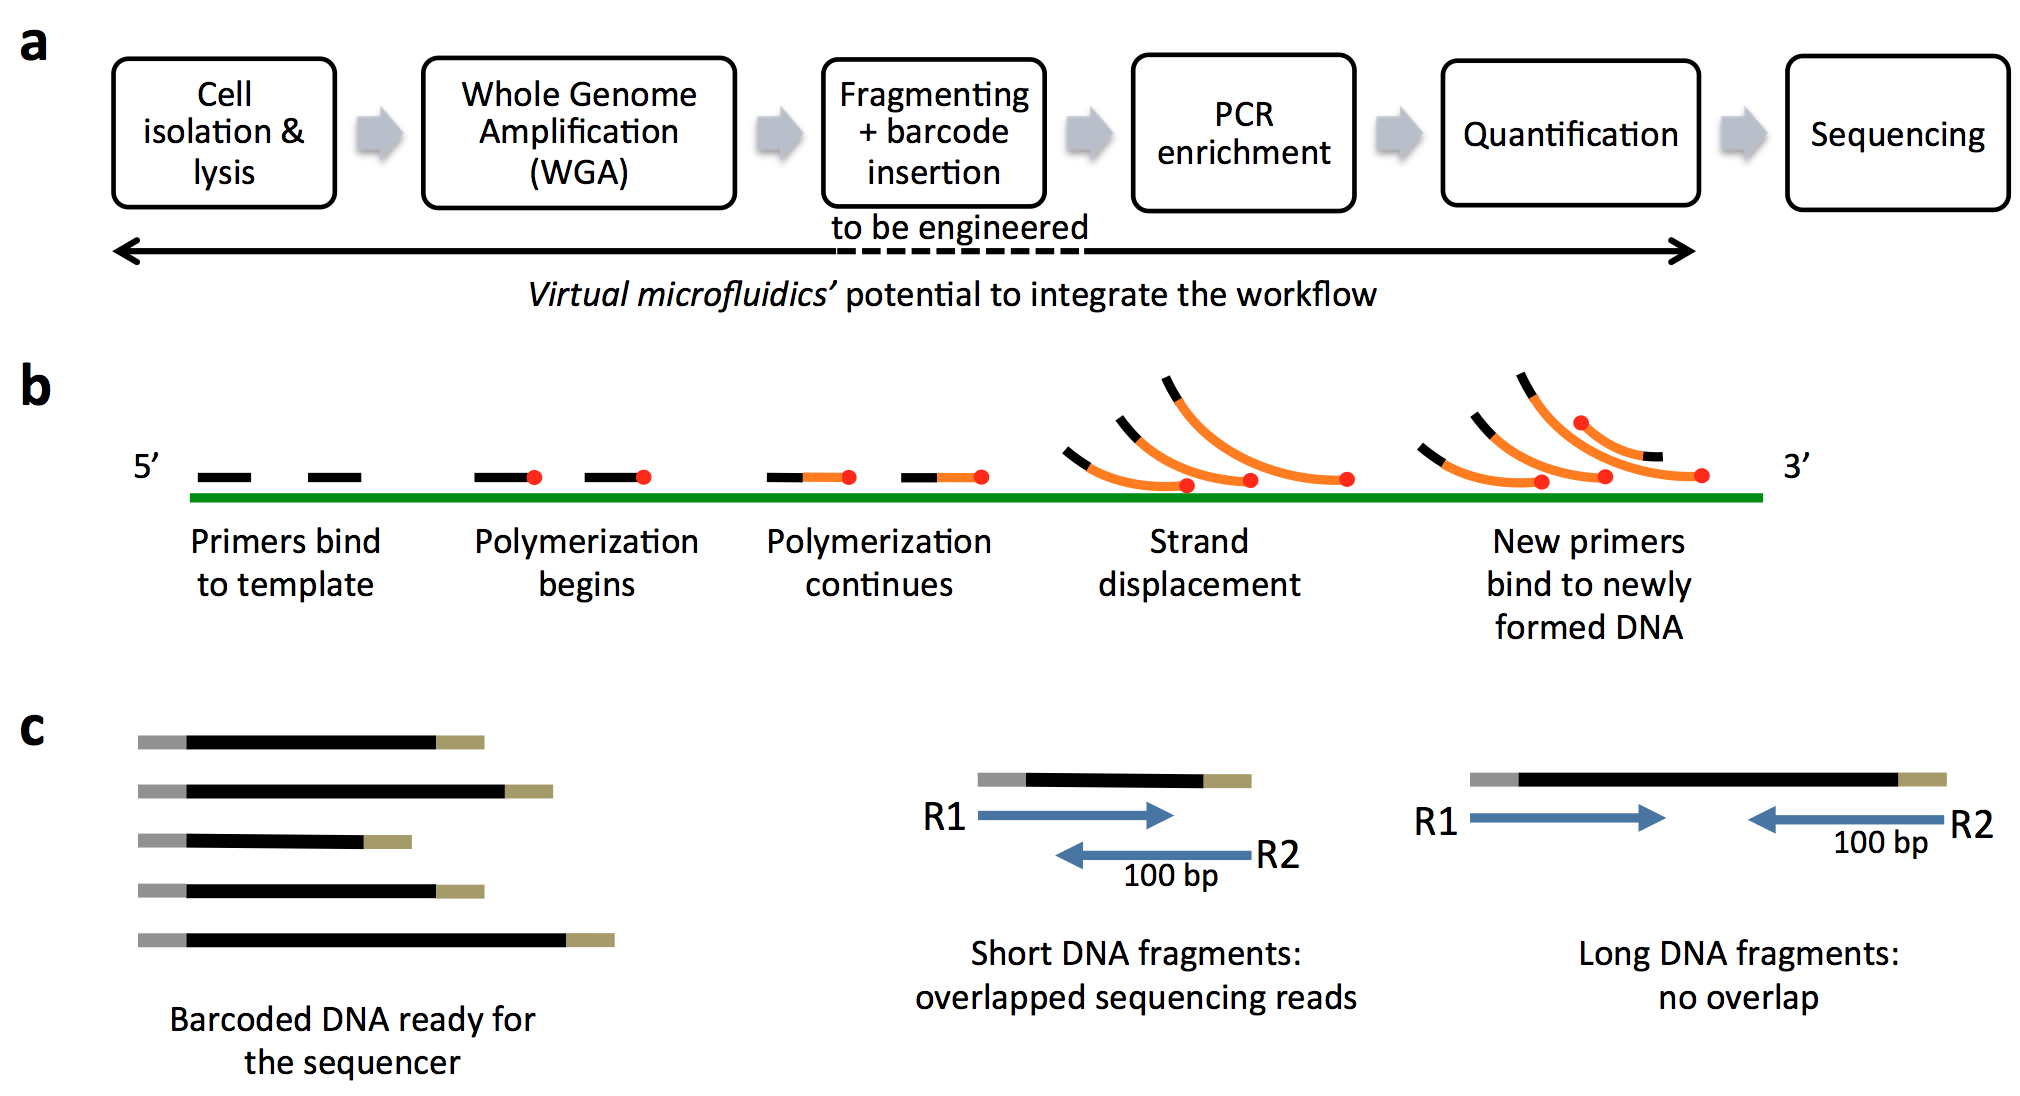
\includegraphics[keepaspectratio,width=\textwidth]{./figures/Introduction_Sequencing}
\caption[An overview of single-cell whole genome sequencing]{An overview of single-cell whole genome sequencing. (a) The single-cell analysis workflow. (b) Multiple displacement amplification (MDA) mechanism. (c) DNA are fragmented, barcoded and sequenced with pair-end sequencing.}
\label{fig:Intro}
\end{figure}

\subsubsection{Cell isolation and lysis} 
Like with single-molecule analysis, the first critical step in single-cell analysis is cell isolation. In order to separate cells of interest, relatively high-throughput technologies were developed recently, such as fluorescent-activated cell sorting (FACS) into multi-well plates \cite{Zhang:2006hq}, high-density microfluidic arrays \cite{Love:2013hf}, engineered lab-on-chip systems \cite{Thorsen:2002dn,Landry:2013dh,deBourcy:2014ji, Marcy:2007ip}, and multi-phase micro-droplet systems \cite{Fu:2015gl,Thorsen:2001td,Morinishi:2015jx,Mazutis:2013wn,Hindson:2013hb} (see Table \ref{tab:singlecellisolation}). %In addition to looking at the cells directly with FISH (fluorescent in situ hybridization) \cite{Kwon:2013wq,Raj:2009ds} and microarrays \cite{Neumann:2010il}. 

\begin{table}[ht!]
\caption{A comparison of single-cell isolation technologies}
\label{tab:singlecellisolation}
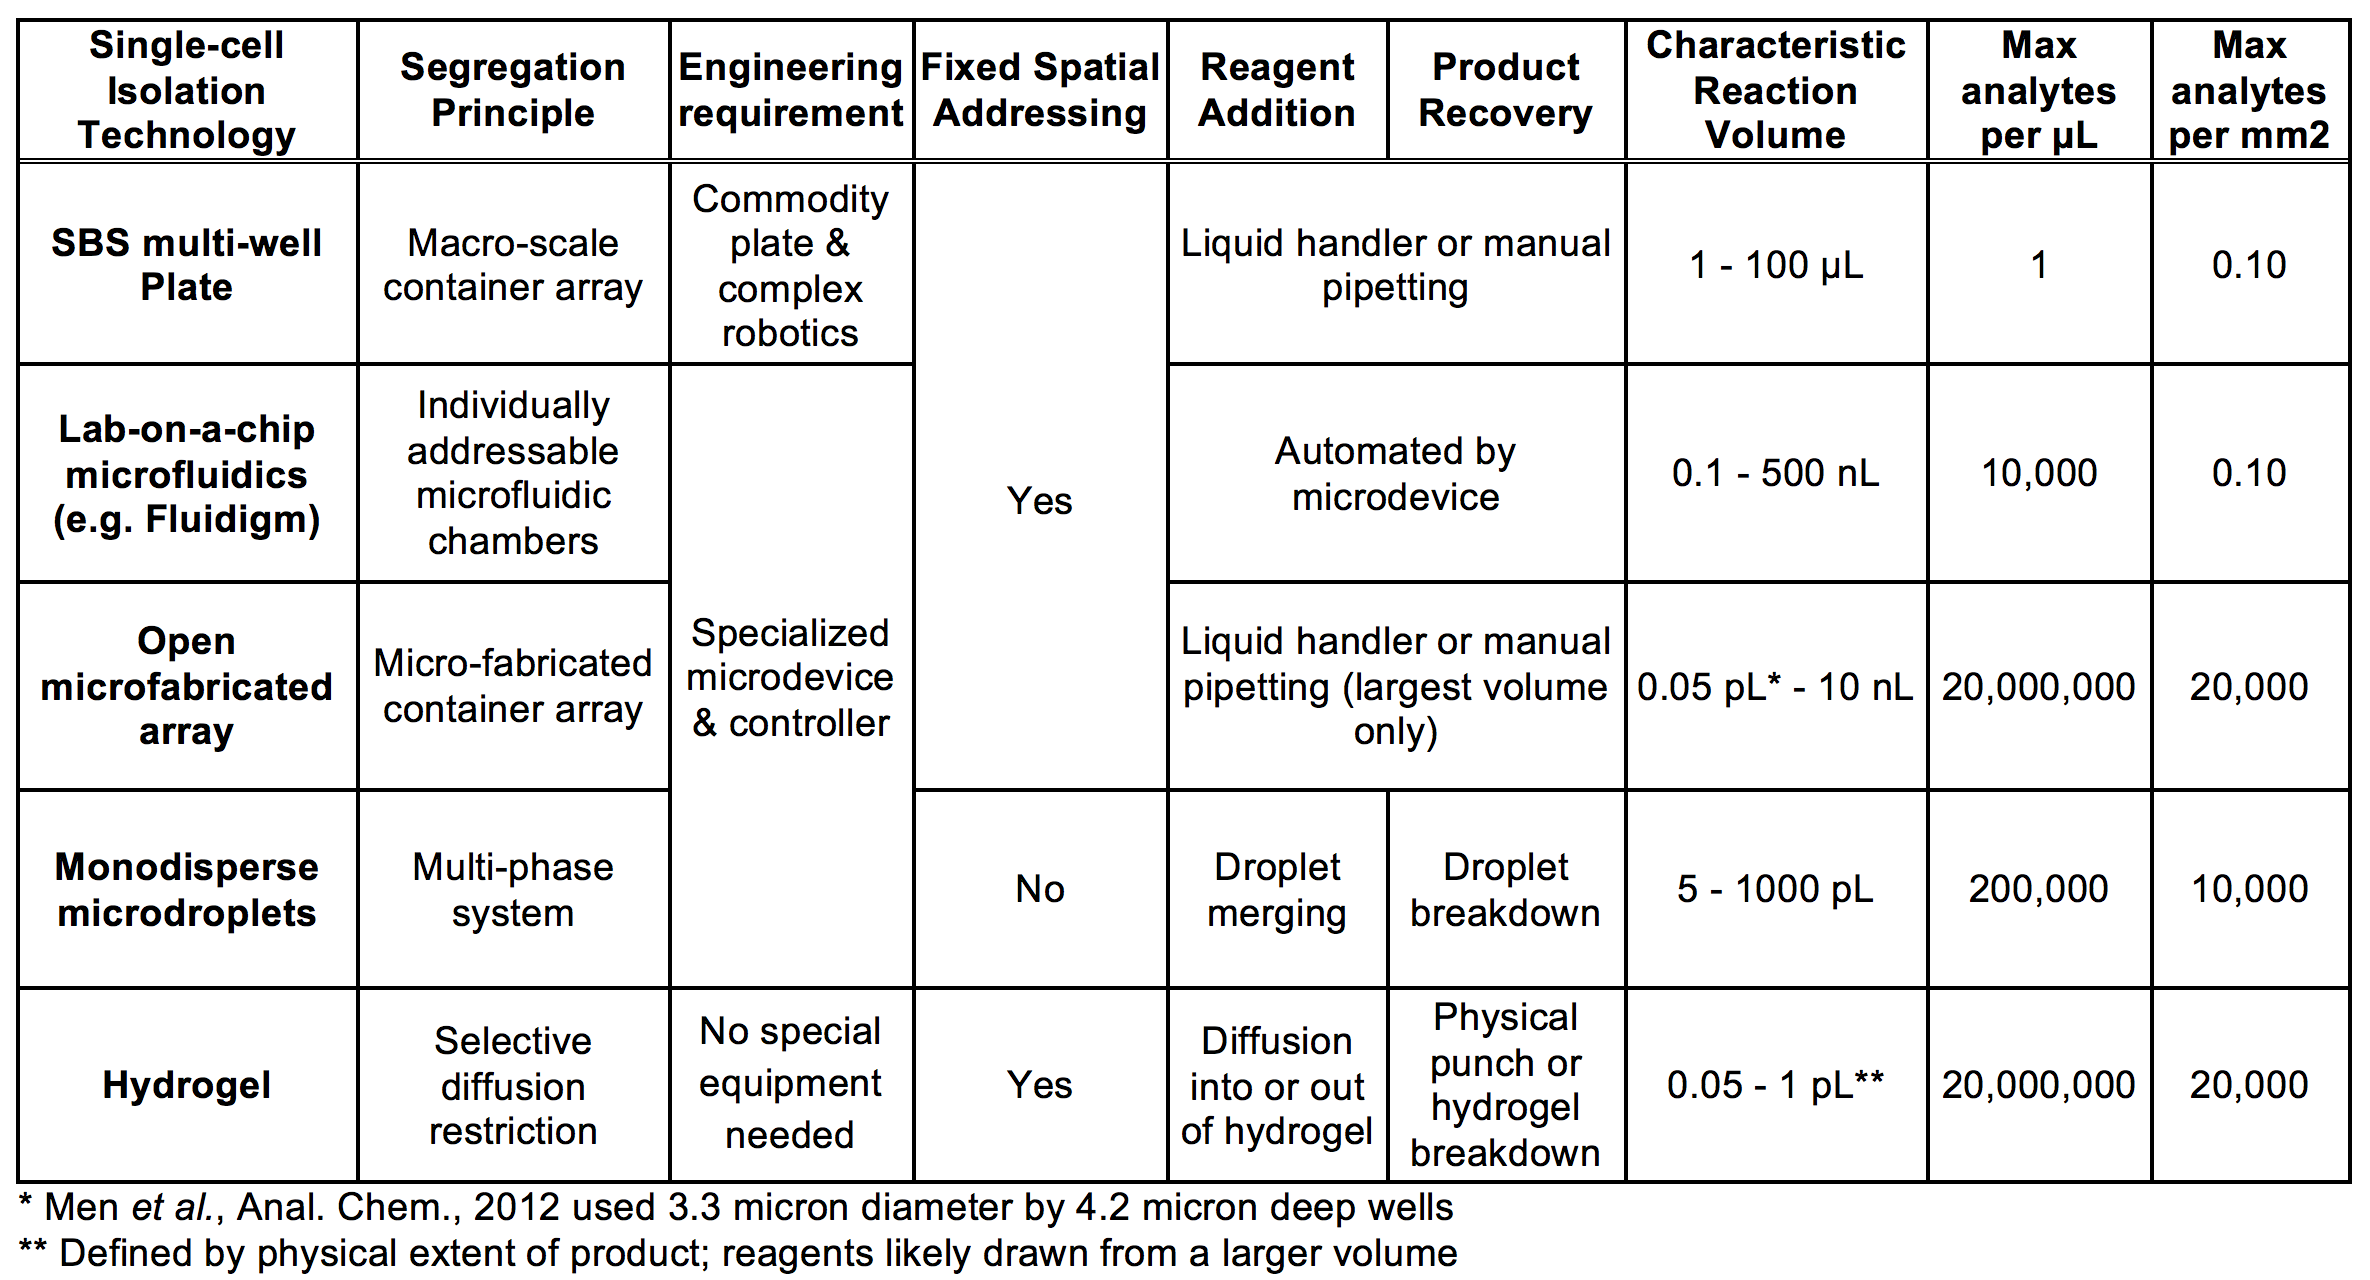
\includegraphics[width=\linewidth]{./figures/TechnologyComparisons.png}
\end{table}

Currently, the most commonly used method for cell isolation is FACS. FACS automates the process of single-cell isolation of identifiable subpopulations. The cells being sorted need to have differentiating light-scattering characteristics, express certain fluorescent markers, or to be stained by fluorescent antibodies or DNA binding dyes. Studies have used FACS with DNA binding dyes to detect and localize genetic abnormalities such as whole chromosomal deletions and aneuploidy on single cells \cite{Trask:2002iy}. The human cell size (10$\mu$m $\sim$ 20$\mu$m in diameter) and surface properties make it a suitable sample for FACS. However, it is difficult to achieve a similar success rate when separating environmental microorganisms ($\sim$ 1$\mu$m). Environmental microbial samples have a range of morphological shapes and this may result in a biased selection by fluorescent scattering, which contributes to a possible uneven representation of taxa obtained through single-cell analysis using FACS compared to bulk metagenomic sequencing. Sample preparations involving FACS, plate/well transfer, and dilution greatly increase the possibility of exogenous DNA contaminations from the lab environment \cite{Woyke:2011eg}. In the case of single-cell whole genome amplification, one single molecule of exogenous DNA can pose great challenges to amplification methods using the random priming mechanism and affect the quality of \textit{de novo} assemblies \cite{Blainey:2011dt}.

To remedy the effect of sample handling, a wide variety of approaches have been explored for the microfluidic compartmentalization of single cells across a large number of small discrete reactors \cite{deBourcy:2014ji,Marcy:2007ip}. However, similar to the current methods for single-molecule analysis, existing methods require complex instrumentation and are labor intensive if set up in-house. In addition to the characteristics desired as in single-molecule assays, single-cell studies often require the compartment access for the addition and product removal of reagents and samples. A recent development of a microfluidic system that incorporates DNA purifying capability for processing microbial isolates may solve the reagent addition and retrieval problem but it is not easily accessible and scalable to single-cell resolution \cite{Kim:2017gy}. The operation of open microarray/microwells requires a specialized liquid handler such as Echo^{\textregistered} (Labcyte Inc.) and CellCelector\textsuperscript{TM} (Automated Lab Solutions). Emulsion droplet systems pose challenges in reagent addition and sample retrieval after the droplet formation. This approach is positioned well to produce a large number of picoliter partitions easily for digital counting in a single-molecule analysis that doesn't require follow up Sanger or whole genome sequencing (WGS). A recent development utilizing droplets as partitions for a single human genome WGA still requires FACS sorting or mouth pipetting for cell isolation \cite{Fu:2015gl}. 

The challenges in the single-microbe analysis are distinct from its mammalian counterpart. The difficulty in culturing prevents us from obtaining single colonies on an agar plate that provides enough starting material for sequencing (nanograms of DNA for Illumina benchtop procedures). Here is where single microbe Whole Genome Amplification (WGA) comes into play. WGA can amplify the femtograms of genomic DNA from a single microbe to nanograms (See next section on WGA for more detail). However, single microbial WGA faces numerous challenges, including low isolation efficiency and a high chance of contamination. In addition, microbial communities consist of organisms with diverse physiologies, meaning that a universal lysis strategy that works for all types is difficult due to the diverse chemical compositions of cell walls. Most lysis methods are developed for bulk samples, which may not be suitable at the single-cell level if the lysis efficiency is low \cite{Blainey:2013dp}. The undesired consequences of incomplete lysis might result in DNA locus damage and undetected microbial species. 

Alkaline lysis is the most common method for single microbe lysis today and it was first described for single cells by Raghunathan \textit{et al.} \cite{Raghunathan:2005fg}. Other supplementary methods include heat lysis, repeated freeze-thaw \cite{Swan:2011hb,Fleming:2011dv}. But the lysis success rates (obtaining pure single amplified genomes after WGA) vary widely and are often below 40\%  \cite{Stepanauskas:2012ja}. One particular type of microbes that does not lyse well in alkaline is environmental extremes, such as \textit{M. ruber} that was found in hot springs with alkaline pH \cite{NOBRE:1996ke}. On the other hand, Fleming \textit{et al.} discussed that the best strategy might be using a cocktail of enzymes that provide efficient but gentle lysis on the entire microbe types present \cite{Fleming:2011dv}. But enzymatic cocktail unavoidably contains small fragments of DNA lodged in the enzymes themselves, which become contaminants through the WGA step. The enzymatic cocktail for one single cell in isolation is often excessive and might not be compatible with downstream WGA method. And it is difficult to purify such a low quantity of unamplified genomic DNA. Consequently, an effective, adaptable and clean method to enable high-throughput single-microbe isolation and lysis is needed. % Linda says fix grammer 

Cell isolation and lysis for mammalian cells is less technically challenging due to their relatively large cell size and the absence of the cell wall. The lipid bilayer cell membrane can be easily dissolved in a dilute solution of detergent, such as Triton-100X and NP-40. The enzymatic digestion and DNA deproteination methods have been widely implemented and optimized \cite{Zong:2012bs,Fu:2015gl,Leung:2016vx,Chen:2017hq,Dean:2002us}. However, it was recently discovered that many single-cell studies could be confounded by the poor data quality caused by the DNA damage after cell lysis when biological \say{variations} are in fact extensive technical biases and errors \cite{Chen:2017hq,Chen:2017dq}. For sensitive applications such as measuring the single-nucleotide variations (SNVs) in cancer cells, treating the genomic DNA with uracil-DNA glycosylase to eliminate cytosine-deaminated uracil bases can reduce a significant amount of false-positive C-to-T SNVs \cite{Chen:2017hq,Rohland:2015uk}. 

\subsubsection{Whole Genome Amplification (WGA)}
One of the most critical steps to analyze genomes of single cells is the whole genome amplification. Currently, the prevalent short-read library preparation and sequencing technologies require nanograms ($10^{-9}$ g) of input DNA for on bench procedures, while the genome of a single cell ranges from femtograms ($1.7 \times 10^{-15}$ g, \textit{Prochlorococcus} MED4) to picograms ($6 \times 10^{-12}$ g, human diploid). Thurs, WGA is needed to replicate the genomic DNA from a single-cell to approximately $10^3 \sim 10^6$ fold. During the WGA process, artifacts and technical errors such as low physical genome coverage, non-uniform coverage due to GC\% bias, false-positive (FP) errors and false-negative errors are often introduced. Achieving a high physical coverage of the genome with a low error rate is crucial for calling mutations accurately at the same regions of multiple single cells. There is a need for WGA method improvement that provide high-quality single-cell WGA data in above-mentioned criteria.

Multiple Displacement Amplification (MDA) \cite{Dean:2002us} is a well-characterized WGA method commonly used to enable single-cell genome sequencing \cite{Marcy:2007il,Fu:2015gl,Zhang:2006hq,Raghunathan:2005fg,Pamp:2012cj,Dodsworth:2013ih,Hess:2011gu}. MDA uses $\Phi$29 polymerase with a strong strand displacement property and random exonuclease-resistant 6 bp primers to produce longer than 12 kbp amplification products at $30^{\circ}$C (Fig. \ref{fig:Intro}b). MDA provides greater genome coverage than the PCR-based methods such as degenerate oligonucleotide primed PCR (DOP-PCR) and lower error rate than \textit{Taq} and \textit{Bst} owing to the high fidelity of $\Phi$29 polymerase \cite{Dean:2002us}. However, the exponentially amplified genome through MDA has regions that are overrepresented and this bias positively correlates with the fold of amplification \cite{deBourcy:2014ji}. In addition, the random priming nature allows DNA amplification on any exogenous DNA contaminants, posing a threat in raising the false-positive rate in new genome discovery. 

Recent technology innovations have been focused on improving MDA performance by varying methods of physical partitions. It has been shown that contaminating DNA was largely eliminated by moving MDA from microliter reaction volumes in tubes to a microfluidic format that used nanoliter volumes \cite{deBourcy:2014ji}. The MDA amplification gain is also limited by the nanoliter volume, thus improving its coverage uniformity. The trend of using sub-microliter partitions lead to the development of emulsion WGA (eWGA) \cite{Fu:2015gl} and Nanodrop MDA \cite{Leung:2016vx}. In eWGA, a single cell is FACS sorted and lysed, then randomly distributes in a large number ($10^5$) of picoliter droplets. Each droplet contains zero to a few fragments of DNA that go through MDA reaction. The results showed improved uniformity and high coverage at the amplification gain of 2 \times $10^6$ for human cells. This improvement is made possible by isolating different parts of the genome during MDA. Thus, this way, the over-amplified fragments would not compete globally with fragments in different droplets that have a late start in MDA. This results in a more uniform amplification depth that improves copy number variations calling accuracy. Nanodrop MDA utilizes commercially available piezoelectric non-contact liquid dispenser to deposit nanoliter-ranged drops sequentially onto a planar substrate and each drop's single-cell occupancy depends on Poisson loading. MDA reagents are added to drops containing single cells in the same way and each 100 nL reaction is covered with mineral oil to prevent evaporation. Both eWGA and Nanodrop methods have shown improvements in terms of data quality in genome coverage percentage and coverage uniformity. But both methods still rely on FACS sorting or liquid dispensing and the rate of artifacts formed in MDA was not characterized. High level of chimeric DNA rearrangements (artifacts) can lead to inaccurate genome structural variation analysis but are rarely analyzed in single-cell technology development. We will discuss in depth on this subject in Chapter 4 and how it can impact microbial \textit{de novo} assembly, investigating mutational mosaicism in neurons, and single-cell cancer research. 

%Quantifying the mutation rate and the mutation heterogeneity in cancer are difficult tasks to tackle. These genomic changes are summarized into 3 main categories: single nucleotide variations (SNVs), Copy Number Variations (CNVs), and structural variations. Among those, genome Structural Variations (SV)(including inversion, translocation, duplication) are an important source of cancer cell heterogeneity and brain developmental diseases but remain technical challenging to detect from bulk sequencing \cite{Norris:2016ec}. There is an unmet need for clinical assays that can cheaply and rapidly profile SVs in solid tumors in a low-input or single-cell resolution \cite{Macintyre:2016hw}. The mutation definition in this context includes a wide range of heritable changes in the nucleotide sequence of DNA, such as single nucleotide point mutation, gene insertion, deletion, rearrangements and large-scale chromosomal abnormalities (trisomy, inversion, translocation, etc). 

In addition to improving the experimental setup for MDA, efforts have been made to develop new WGA chemistry that linearly amplifies the genome to reduce biased coverages the dependence on complex instruments \cite{Zong:2012bs,Chen:2017hq}. The most recent method LIANTI (Linear Amplification via Transposon Insertion) utilizes direct transposon insertion and \textit{in vitro} transcription to linearly amplify RNA copies of the genome. This method eliminates the random non-specific priming used in traditional MDA method and has shown to improve coverage uniformity and reduce the false-positive rate in calling single nucleotide variations. The reduction of the error rate is due to linear amplification's random error position on the same template. By sequencing single cells to a high depth (30$\times$), amplification error would be corrected, which leads to less false positive calls. LIANTI has a huge potential for its wide adoption as the next generation of WGA method. According to the analysis in chapter 4, a majority (70\%) of LIANTI's sequencing reads contain barcode information and poor quality reads. A large portion of sequencing effort is wasted as a result (\$2500 $\times$ 70\% = \$1750 wasted per cell in sequencing cost). More work needs to be done to integrate the transposon barcode insertion and its downstream library preparation.

After WGA, purified DNA will go through library preparation - fragmentation and barcode insertion. Accurately purified and quantified libraries, in terms of both size ranges and quantities, will be loaded onto the sequencer (Fig. \ref{fig:Intro}d). 
 
Overall, the single-cell sequencing process from having cells in suspension to obtaining sequencing data is highly fragmented in terms of technology implementation. eWGA and LIANTI have to rely on traditional FACS sorting or mouth pipetting while Nanodrop requires sequential depositions for both cell isolation and reagents addition. Efforts have been made to integrate library preparation in microfluidic chips \cite{Kim:2017gy} and to package cell isolation and WGA in a commercially available droplet system (10X Genomics). Both examples are either cumbersome to implement or expensive to purchase. For 10X Genomics, for instances, it costs \$ 100K per machine unit. Researchers working in microbial discovery and oncology studies are looking for ways to conduct single-cell sequencing with an economically reasonable and technically manageable method for a large number of single cells. Independent innovations addressing different stages of single-cell sequencing will push the field forward in small steps. Ideally, an integrated approach that provides an accessible platform to streamline the process while produces high-quality data is needed to realize single-cell sequencing's huge potential in scientific discovery and biomedical field. 

\section{\textbf{\textit{Virtual Microfluidics}} for
digital quantification and single-cell sequencing}
In the introduction, we reviewed the increasing scientific and biomedical need for single-molecule and single-cell analysis and their current technology landscape. Much improvement is needed to bridge the gap between the current technology state and the wide adoption of the method. The necessary improvement areas I have discussed include high-throughput, the data quality, the ease of implementation, optical enrichment properties and the process integration. Thus, I developed the method \textit{virtual microfluidics} to make an improvement in above-mentioned areas and to help push the single-molecule and single-cell analysis fields forward (Fig. \ref{fig:VM1}). 

\begin{figure}[ht!]
\centering
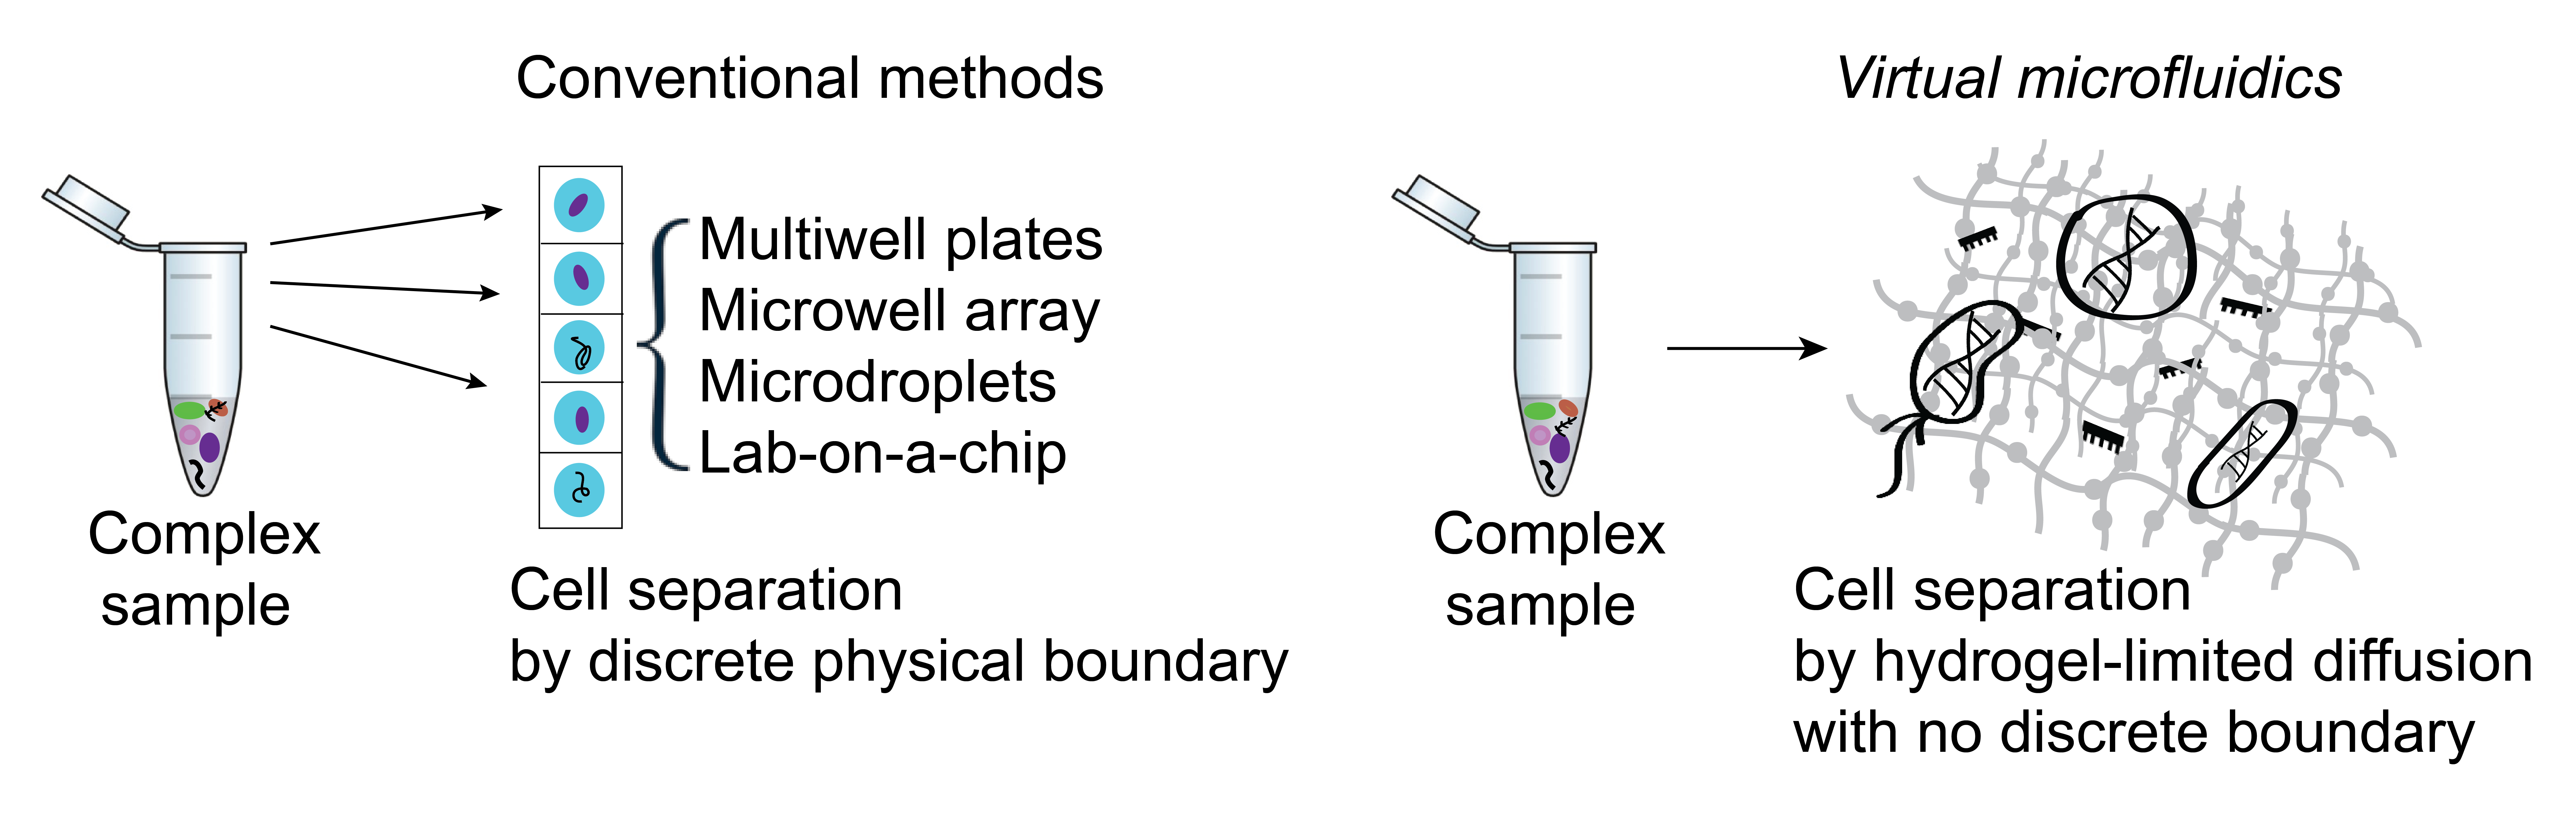
\includegraphics[keepaspectratio,width=1\textwidth]{./figures/Thesis-20.png}
\caption[Conventional methods vs. \textit{virtual microfluidics}]{Conventional methods vs. \textit{virtual microfluidics}. Conventional single-cell analysis methods
require discrete physical boundaries. \textit{Virtual microfluidics} relies on hydrogel-limited diffusion to compartmentalize templates and reaction products.}
\label{fig:VM1}
\end{figure}

Single-molecule and single-cell studies require individual molecules or cells separated in partitions. But instead of creating physical partitions to isolate cells, we decided to build \say{invisible} dividers around them. Passive segregation of single molecules and the product of genome amplification would be able to facilitate the genomic analysis of thousands of nucleic acids in parallel. In order to achieve this, a porous structure that is able to fix many molecules and provide an aqueous environment for DNA amplification was chosen. Thus, the \textit{virtual microfluidics} system was created to enable single-cell WGA \textit{en masse} in poly(ethylene glycol) (PEG) hydrogel. The hydrogel properties allow reagent exchange by diffusion, imaging accessibility, product retrieval easiness and improved WGA performances using MDA compared to instrumentation-based methods. \textit{Virtual microfluidics} is also a versatile and compatible platform to integrate PCR, MDA and in-gel library preparation methods, which holds great promise in integrating single-cell analysis field and pushing the wider adoption of the technology (Fig. \ref{fig:FigAbstract}) . 

\begin{figure}[ht!]
\centering
\includegraphics[keepaspectratio,width=1\textwidth]{./figures/SolidPhaseWGAvsTraditional}
\caption[A graphical abstract of the \textit{virtual microfluidics} technique]{A graphical abstract of the \textit{virtual microfluidics} technique.}
\label{fig:FigAbstract}
\end{figure}

In chapter 2, I will characterize \textit{virtual microfluidics} in quantifying DNA targets for single-molecule analysis and demonstrated its improvement in the ease of implementation and its wide dynamic range in quantifying DNA targets. In chapter 3, \textit{virtual microfluidics} is applied to mixed cultures of bacteria and the human gut microbiome. It produces single amplified genomes with excellent coverage uniformity and markedly reduced chimerism compared with liquid MDA reactions. We demonstrate single-cell sequencing on human gut microbiome samples and obtain 117 pure single draft genomes that enabled the identification of more than 10,000 horizontally transferred genes that have unique population-specific and individual-specific features \cite{Brito:2016cd}. In chapter 4, I will show how \textit{virtual microfluidics} reduces the amount of chimera artifacts from MDA on single amplified human genomes compared to above-mentioned technologies. 
 
The results described in chapter 2 and 3 have been published as Xu \textit{et al.} Nature Methods. 2016.

The single-cell dataset generated from the human gut microbiome contributed to the publication of Brito \textit{et al.} Nature. 2016.

